\documentclass[12pt]{report}
\usepackage{graphicx}
\usepackage{subfig}

\begin{document}

\title{Homework 0 - Writeup}
\author{Tim Delisle and Sam Raudabaugh}
\date{08/26/2015}
\maketitle

\begin{figure}
\centering
\subfloat[sepal wid vs sepal len]{
  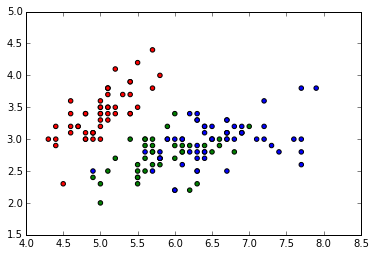
\includegraphics[width=45mm]{figures/1.png}
}
\subfloat[petal len vs sepal len]{
  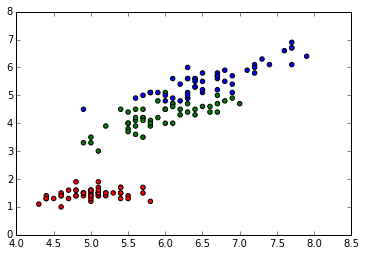
\includegraphics[width=45mm]{figures/2.png}
}
\subfloat[petal wid vs sepal len]{
  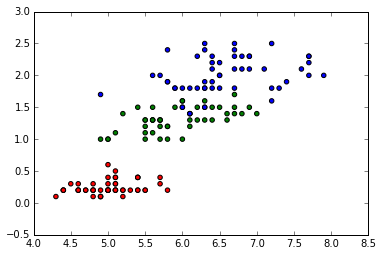
\includegraphics[width=45mm]{figures/3.png}
}
\hspace{0mm}
\subfloat[petal len vs sepal wid]{
  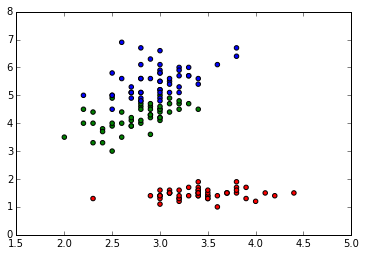
\includegraphics[width=45mm]{figures/4.png}
}
\subfloat[sepal len vs sepal wid]{  
  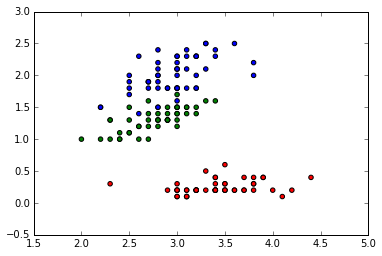
\includegraphics[width=45mm]{figures/5.png}
}
\subfloat[sepal wid vs petal len]{
  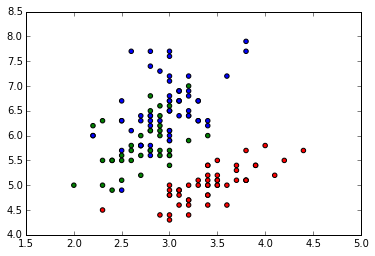
\includegraphics[width=45mm]{figures/6.png}
}
\hspace{0mm}
\subfloat[petal wid vs petal len]{
  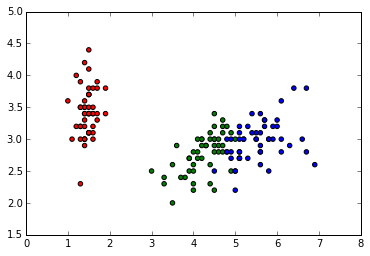
\includegraphics[width=45mm]{figures/7.png}
}
\subfloat[petal wid vs petal len]{  
  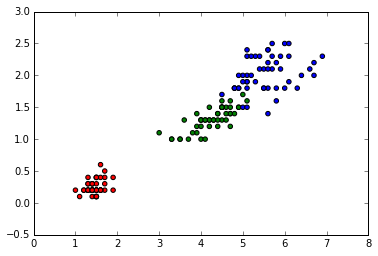
\includegraphics[width=45mm]{figures/8.png}
}
\subfloat[sepal len vs petal len]{
  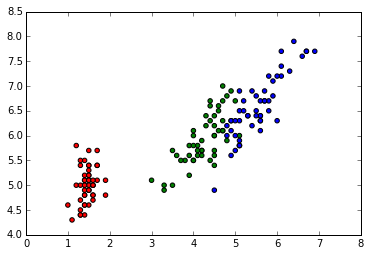
\includegraphics[width=45mm]{figures/9.png}
}
\hspace{0mm}
\subfloat[sepal wid vs petal wid]{
  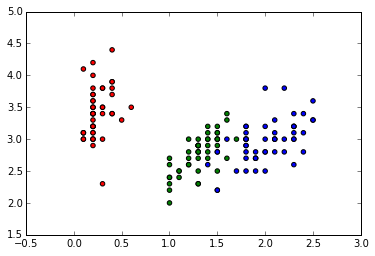
\includegraphics[width=45mm]{figures/10.png}
}
\subfloat[petal len vs petal wid]{  
  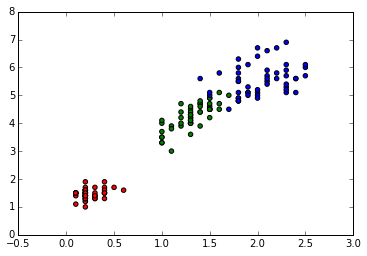
\includegraphics[width=45mm]{figures/11.png}
}
\subfloat[sepal len vs petal wid]{
  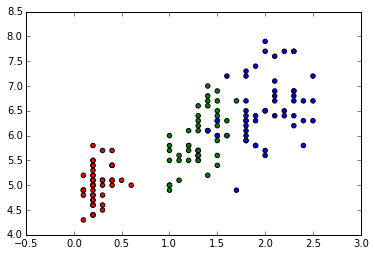
\includegraphics[width=45mm]{figures/12.png}
}
\caption{caption}
\end{figure}

\end{document}
